\documentclass{beamer}

\mode<presentation>
{
  \usetheme{Frankfurt}
  \usecolortheme{orchid}
  \setbeamercovered{invisible}
  \setbeamertemplate{footline}[frame number]
}

\usepackage[english]{babel}
\usepackage[latin1]{inputenc}
\usepackage{times}
\usepackage[T1]{fontenc}
\usepackage{tikz}
\usepackage{array}
\usepackage{cancel}


\usetikzlibrary{shapes,backgrounds}

\def\multiset#1#2{\ensuremath{\left(\kern-.3em\left(\genfrac{}{}{0pt}{}{#1}{#2}\right)\kern-.3em\right)}}

\def\blue{\color{blue}~}
\def\black{\color{black}~}
\def\bl[#1]#2{\begin{block}{#1}#2\end{block}}
\def\integers{\mathbb{Z}}
\def\enumb{\begin{enumerate}}
\def\enume{\end{enumerate}}
\def\itemb{\begin{itemize}}
\def\iteme{\end{itemize}}


\usepackage{remreset}
\makeatletter
\@removefromreset{subsection}{section}
\makeatother
\setcounter{subsection}{1}

\title{Discrete Mathematics, Section 001, Fall 2016}
\subtitle{Lecture 13: Functions}

\author[Zsolt]{Zsolt Pajor-Gyulai \\ \texttt{zsolt@cims.nyu.edu}}
\date{October 31, 2016}

\pgfdeclareimage[height=1cm]{NYUlogo}{NYUlogo.jpg}

\institute[NYU] 
{
\normalsize Courant Institute of Mathematical Sciences
}
\titlegraphic{\pgfuseimage{NYUlogo}}

\begin{document}

\begin{frame}
  \titlepage
\end{frame}

\AtBeginSection[]
{
\begin{frame}
\frametitle{Outline}
\tableofcontents[currentsection]
\end{frame}}

\section{Abstract notion of a function}

\begin{frame}{What is a function?}
\underline{Intuitively:} a function is a `rule' or `mechanism' that transforms one quantity into another.
\itemb
\item $f(x)=x^2+4$ takes an integer $x$ and transforms it into the integer $x^2+4$.
\item $g(x)=|x|$ takes the integer $x$ and returns $x$ if $x\geq 0$ and $-x$ if $x<0$.
\iteme

\vspace{0.4cm}

\underline{Abstract sense:} Functions are special types of relations.

\bl[Definition]{A relation $f$ is called a \textbf{function} provided $(a,b)\in f$ and $(a,c)\in f$ imply $b=c$.}
In other words, $f$ is not a function if there are $a,b,c$ such that $(a,b),(a,c)\in f$ but $b\neq c$.
\end{frame}

\begin{frame}{What is a function?}
\bl[Definition]{A relation $f$ is called a \textbf{function} provided $(a,b)\in f$ and $(a,c)\in f$ imply $b=c$.}
For example, consider
\[
f=\{(1,2),(2,3),(3,1),(4,7)\},\qquad g=\{(1,2),(1,3),(4,7)\}.
\]
Here $f$ is a function, but $g$ is not because $(1,2),(1,3)\in g$ but $2\neq 3$.

\center Get used to this by doing Problem 1 on the worksheet.

\end{frame}

\begin{frame}{Functional notation}
\bl[Definition]{A relation $f$ is called a \textbf{function} provided $(a,b)\in f$ and $(a,c)\in f$ imply $b=c$.}

\bl[Definition]{Let $f$ be a function. If $(a,b)\in f$, we write
\[
f(a)=b.
\]}
\only<1>{
By the definition of a function this is unambiguous, as for any object $a$, there is at most one $b$ such that $(a,b)$. }

\uncover<2>{For example, consider
\[
f=\{(1,2),(2,3),(3,1),(4,7)\},\qquad g=\{(1,2),(1,3),(4,7)\}.
\]\vspace{-0.4cm}

\itemb
\item $f(1)=2$, $f(2)=3$, $f(3)=1$, $f(4)=7$ \\but , e.g. $f(10)$ is undefined.
\item $g(1)$ is ambiguous.
\iteme}
\end{frame}

\begin{frame}{Example}
\bl[]{Express the integer function $f(x)=x^2$ as a relation.}

\itemb
\item \underline{Option 1:} List elements
\[
f=\{\dots, (-3,9),(-2,4), (-1,1), (0,0), (1,1), (2,4), (3,9),\dots\}
\]\vspace{0.4cm}
\item \underline{Option 2:} Set-builder notation
\[
f=\{(x,y): x,y\in\mathbb{Z}, y=x^2\}
\]
\iteme

\end{frame}

\section{Domain and Image}

\begin{frame}{Definitions}
\bl[Definition]{Let $f$ be a function. The set of all possible first elements of the ordered pairs in $f$ is called the \textbf{domain} of $f$ and is denoted $\textrm{dom} f$.}
In other words,
\[
\textrm{dom} f=\{a:\exists b, (a,b)\in f\}=\{a:f(a)\textrm{ is defined}\}
\]

\bl[Definition]{Let $f$ be a function. The set of all possible second elements of the ordered pairs in $f$ is called the \textbf{image} of $f$ and is denoted $\textrm{im} f$.}
In other words,
\[
\textrm{im} f=\{b:\exists a, (a,b)\in f\}=\{b: b= f(a)\textrm{ for some $a$}\}
\]
\end{frame}

\begin{frame}{Example}
\itemb
\item Let $f=\{(1,2),(2,3),(3,1),(4,7)\}$. Then
\[
\textrm{dom} f=\{1,2,3,4\},\qquad\textrm{im}f=\{1,2,3,7\}.
\]
\item Let $f=\{(x,y): x,y\in\mathbb{Z}, y=x^2\}$. Then
\[
\textrm{dom} f=\mathbb{Z},\qquad\textrm{im}f=\{y\in\mathbb{Z}: \textrm{$y$ is a perfect square}\}.
\]
\iteme
\center Practice this by doing Problem 2 on the Worksheet.
\end{frame}

\begin{frame}{Yet another notation}
\bl[Definition]{Let $f$ be a function and let $A$ and $B$ sets. We say that $f$ is a function from $A$ to $B$ provided $\textrm{dom}f$=A and $\textrm{im} f\subseteq B$. In this case we write $f:A\to B$ and also say that $f$ is a mapping from $A$ to $B$.}
Saying $f: A\to B$ means three things:
\itemb
\item $f$ is a function.
\item $\textrm{dom}f=A$.
\item $\textrm{im}f\subseteq B$.
\iteme
For example,
\[
\sin:\mathbb{R}\to\mathbb{R},\qquad \sin:\mathbb{R}\to [-1,1]
\]
To show that $f:A\to B$, the above three conditions need to be checked.
\end{frame}

\section{Pictures of functions}

\begin{frame}{The usual function graph}
Graphs provide excellent visualization of functions whose inputs and outputs ar real numbers.
\itemb
\item Note that when $\textrm{dom} f$, $\textrm{im} f\subseteq \mathbb{R}$, then $f\in\mathbb{R}\times\mathbb{R}$.
\item If $f$ is nice enough, the points in $\mathbb{R}\times\mathbb{R}$ that belong to $f$ give a nice curve.
\iteme

E.g., when $f:[0,2]\to \mathbb{R}$ is defined by $f(x)=1-x^2+0.3x^3$,

\begin{figure}
\centering
\begin{tikzpicture}
\draw (0,-0.7) -- (0,1.2); \draw (-1.2,0) -- (3.2,0);
\draw[domain=0:2,smooth,variable=\y]  plot ({\y},{1-(\y)*(\y)+0.3*(\y)*(\y)*(\y)});
\end{tikzpicture}
\end{figure}

This, however, doesn't work when $\textrm{dom} f$ is more complicated, e.g.
\[
f:2^A\to \mathbb{N},\qquad f(B)=|B|
\]
\end{frame}

\begin{frame}{Alternative for finite sets}
Consider $A=\{1,2,3,4,5,6\}$ and $B=\{1,2,3,4,5\}$ and
\[
f:A\to B,\qquad f=\{(1,2),(2,1),(3,2),(4,4),(5,5), (6,2)\}.
\]

\begin{figure}
\centering
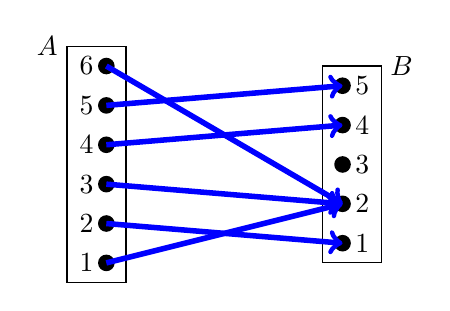
\begin{tikzpicture}
\foreach \x in {1,...,6}
	{\fill[black] (0,0.5*\x-0.5) circle (3pt); 
	\node at (-0.25,0.5*\x-0.5) {\x};}

\draw (-0.5,-0.25) -- (0.25,-0.25) -- (0.25, 2.75) -- (-0.5,2.75) -- (-0.5,-0.25);

\foreach \x in {1,...,5}
	{\fill[black] (3,0.5*\x-0.25) circle (3pt);
	\node at (3.25,0.5*\x-0.25) {\x};}
	
\draw (2.75,0) -- (3.5,0) -- (3.5, 2.5) -- (2.75,2.5) -- (2.75,0);

\draw[line width=2pt,blue,->] (0,0) -- (3,0.75);
\draw[line width=2pt,blue,->] (0,0.5) -- (3,0.25);
\draw[line width=2pt,blue,->] (0,1) -- (3,0.75);
\draw[line width=2pt,blue,->] (0,1.5) -- (3,1.75);
\draw[line width=2pt,blue,->] (0,2) -- (3,2.25);
\draw[line width=2pt,blue,->] (0,2.5) -- (3,0.75);

\node at (-0.75,2.75) {$A$};
\node at (3.75,2.5) {$B$};

\end{tikzpicture}
\end{figure}
From this, it is easy to read off $\textrm{im} f=\{1,2,4,5\}$.
\end{frame}

\begin{frame}
Of course, we can draw arrows for any relations. $f:A\to B$ means that
\itemb
\item There is an arrow from all `dots' in $A$.
\item There is at most one arrow from all `dots in $A$.
\iteme
Consider the same sets as on the previous slide.
\begin{columns}
\column{0.5\textwidth}
\begin{figure}
\centering
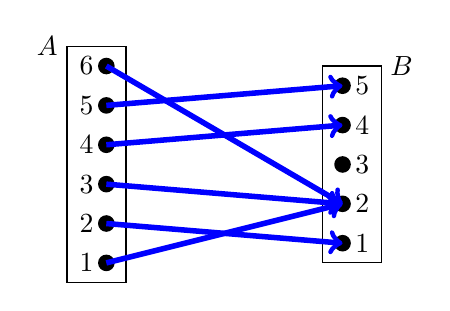
\begin{tikzpicture}
\foreach \x in {1,...,6}
	{\fill[black] (0,0.5*\x-0.5) circle (3pt); 
	\node at (-0.25,0.5*\x-0.5) {\x};}

\draw (-0.5,-0.25) -- (0.25,-0.25) -- (0.25, 2.75) -- (-0.5,2.75) -- (-0.5,-0.25);

\foreach \x in {1,...,5}
	{\fill[black] (3,0.5*\x-0.25) circle (3pt);
	\node at (3.25,0.5*\x-0.25) {\x};}
	
\draw (2.75,0) -- (3.5,0) -- (3.5, 2.5) -- (2.75,2.5) -- (2.75,0);

\draw[line width=2pt,blue,->] (0,0) -- (3,0.75);
\draw[line width=2pt,blue,->] (0,0.5) -- (3,0.25);
\draw[line width=2pt,blue,->] (0,1) -- (3,0.75);
\draw[line width=2pt,blue,->] (0,1.5) -- (3,1.75);
\draw[line width=2pt,blue,->] (0,2) -- (3,2.25);
\draw[line width=2pt,blue,->] (0,2.5) -- (3,0.75);

\node at (-0.75,2.75) {$A$};
\node at (3.75,2.5) {$B$};

\end{tikzpicture}
\end{figure}\vspace{-1.5cm}

\center
\begin{align*}
f=\{&(1,2),(2,1),(3,2),\\
&(4,4),(5,5),(6,2)\}
\end{align*}
 $f:A\to B$
\column{0.5\textwidth}
\begin{figure}
\centering
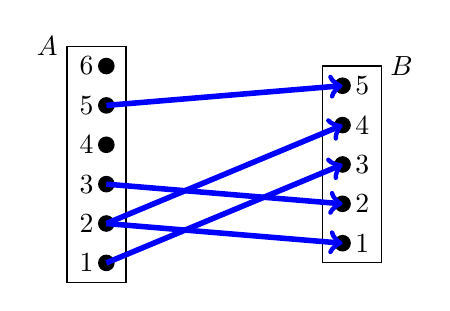
\begin{tikzpicture}
\foreach \x in {1,...,6}
	{\fill[black] (0,0.5*\x-0.5) circle (3pt); 
	\node at (-0.25,0.5*\x-0.5) {\x};}

\draw (-0.5,-0.25) -- (0.25,-0.25) -- (0.25, 2.75) -- (-0.5,2.75) -- (-0.5,-0.25);

\foreach \x in {1,...,5}
	{\fill[black] (3,0.5*\x-0.25) circle (3pt);
	\node at (3.25,0.5*\x-0.25) {\x};}
	
\draw (2.75,0) -- (3.5,0) -- (3.5, 2.5) -- (2.75,2.5) -- (2.75,0);

\draw[line width=2pt,blue,->] (0,0) -- (3,1.25);
\draw[line width=2pt,blue,->] (0,0.5) -- (3,0.25);
\draw[line width=2pt,blue,->] (0,0.5) -- (3,1.75);
\draw[line width=2pt,blue,->] (0,1) -- (3,0.75);
\draw[line width=2pt,blue,->] (0,2) -- (3,2.25);
%\draw[line width=2pt,blue,->] (0,2.5) -- (3,0.75);

\node at (-0.75,2.75) {$A$};
\node at (3.75,2.5) {$B$};

\end{tikzpicture}
\end{figure}\vspace{-1.5cm}

\center
\begin{align*}
g=\{&(1,3),(2,1),(2,4),\\
&(3,2),(4,4),(5,5)\}
\end{align*}
Not $g:A\to B$.
\end{columns}
\end{frame}

\section{Inverse functions}

\begin{frame}{Inverse as a relation}
Recall the inverse of a relation:
\[
R^{-1}=\{(x,y): (y,x)\in R\}
\]
Is the inverse of a function also a function? $\to$ Nope
\[
A=\{1,2,3,4,5\},\qquad B=\{6,7,8,9,10\}
\]\vspace{-0.5cm}
\begin{columns}
\column{0.5\textwidth}
\begin{figure}
\centering
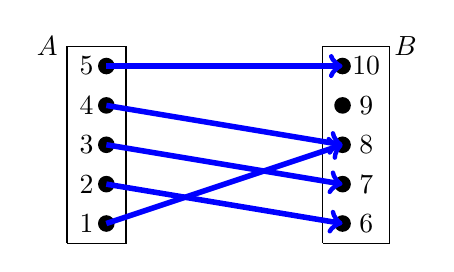
\begin{tikzpicture}
\foreach \x in {1,...,5}
	{\fill[black] (0,0.5*\x-0.5) circle (3pt); 
	\node at (-0.25,0.5*\x-0.5) {\x};}

\draw (-0.5,-0.25) -- (0.25,-0.25) -- (0.25, 2.25) -- (-0.5,2.25) -- (-0.5,-0.25);

\foreach \x in {6,...,10}
	{\fill[black] (3,0.5*\x-3) circle (3pt);
	\node at (3.3,0.5*\x-3) {\x};}
	
\draw (2.75,-0.25) -- (3.6,-0.25) -- (3.6, 2.25) -- (2.75,2.25) -- (2.75,-0.25);

\draw[line width=2pt,blue,->] (0,0) -- (3,1);
\draw[line width=2pt,blue,->] (0,0.5) -- (3,0);
\draw[line width=2pt,blue,->] (0,1) -- (3,0.5);

\draw[line width=2pt,blue,->] (0,1.5) -- (3,1);
\draw[line width=2pt,blue,->] (0,2) -- (3,2);
%\draw[line width=2pt,blue,->] (0,2.5) -- (3,0.75);

\node at (-0.75,2.25) {$A$};
\node at (3.8,2.25) {$B$};

\end{tikzpicture}
\end{figure}\vspace{-0.5cm}
\begin{align*}
f=\{&(1,8), (2,6), (3,7),\\
& (4,8), (5,10)\}
\end{align*}
\column{0.5\textwidth}
\begin{figure}
\centering
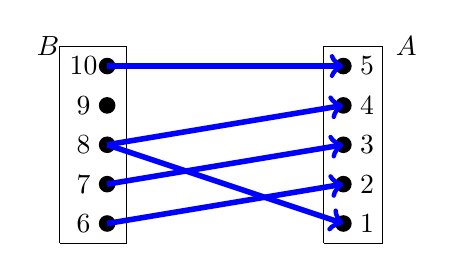
\begin{tikzpicture}
\foreach \x in {6,...,10}
	{\fill[black] (0,0.5*\x-3) circle (3pt); 
	\node at (-0.3,0.5*\x-3) {\x};}

\draw (-0.6,-0.25) -- (0.25,-0.25) -- (0.25, 2.25) -- (-0.6,2.25) -- (-0.6,-0.25);

\foreach \x in {1,...,5}
	{\fill[black] (3,0.5*\x-0.5) circle (3pt);
	\node at (3.3,0.5*\x-0.5) {\x};}
	
\draw (2.75,-0.25) -- (3.5,-0.25) -- (3.5, 2.25) -- (2.75,2.25) -- (2.75,-0.25);

\draw[line width=2pt,blue,->] (0,0) -- (3,0.5);
\draw[line width=2pt,blue,->] (0,0.5) -- (3,1);
\draw[line width=2pt,blue,->] (0,1) -- (3,1.5);
\draw[line width=2pt,blue,->] (0,1) -- (3,0);
%\draw[line width=2pt,blue,->] (0,1.5) -- (3,1);
\draw[line width=2pt,blue,->] (0,2) -- (3,2);
%\draw[line width=2pt,blue,->] (0,2.5) -- (3,0.75);

\node at (-0.75,2.25) {$B$};
\node at (3.8,2.25) {$A$};

\end{tikzpicture}
\end{figure}\vspace{-0.5cm}
\begin{align*}
f^{-1}=\{&(8,1), (6,2), (7,3),\\
& (8,4), (10,5)\}
\end{align*}
\end{columns}
\end{frame}

\begin{frame}{One to one functions}
We would like to characterize those functions whose inverse is also a function.
\bl[Definition]{A function $f$ is called \textbf{one to one} provided that, whenever $(x,b), (y,b)\in f$, we must have $x=y$.}
 In other words, $x\neq y$, then $f(x)\neq f(y)$.
 
 \center{Do the first half of Problem 4 on the worksheet!}
\end{frame}

\begin{frame}
\bl[Proposition]{Let $f$ be a function. The inverse relation $f^{-1}$ is a function if and only if $f$ is one to one.}
\begin{proof}
~~~~First suppose $f^{-1}$ is a function. Assume $(x,b),(y,b)\in f$, then we have $(b,x),(b,y)\in f^{-1}$ and by the definition of a function, we have that $x=y$. This proves that $f$ is one to one.

~~~~Now suppose $f$ is one to one. Assume $(b,x),(b,y)\in f^{-1}$, then $(x,b), (y,b)\in f$ and by $f$ being one-to-one, we see $x=y$. This proves that $f^{-1}$ is a function.
\end{proof}
\center Now do the second part of Problem 4 on the worksheet.
\end{frame}

\begin{frame}
\bl[Proving a function is one to one]{To show that $f$ is one-to-one:
\itemb
\item \textbf{Direct Method:} Suppose $f(x)=f(y)$.$\dots$ Therefore $x=y$ and $f$ is one-to-one.
\item \textbf{Contrapositive method:} Suppose $x\neq y$. $\dots$ Therefore $f(x)\neq f(y)$ and $f$ is one-to-one.
\item \textbf{Contradiction method:} Suppose $f(x)=f(y)$ but $x\neq y$. $\dots$ $\Rightarrow\Leftarrow$ and $f$ is one-to-one.
\iteme}
\end{frame}

\begin{frame}
\bl[Example] {Let $f:\mathbb{Z}\to\mathbb{Z}$ defined by $f(x)=3x+4$. Then $f$ is one-to-one.}
\begin{proof}
Suppose $f(x)=f(y)$. Then $3x+4=3y+4$. Substracting $4$ from both sides gives $3x=3y$. Dividing both sides by $3$ gives $x=y$. Therefore $f$ is one-to-one.
\end{proof}

\bl[Example] {Let $f:\mathbb{Z}\to\mathbb{Z}$ defined by $f(x)=x^2$. Then $f$ is not one-to-one.}
\begin{proof}
Notice that $f(3)=f(-3)=9$, but $3\neq -3$ and thus $f$ is not one to one.
\end{proof}
\end{frame}

\begin{frame}{A more focused question}
\bl[]{\textbf{Q}: If $f:A\to B$, when is it true that $f^{-1}:B\to A$?}\vspace{-0.5cm}

\begin{columns}
\column{0.5\textwidth}
\begin{figure}
\centering
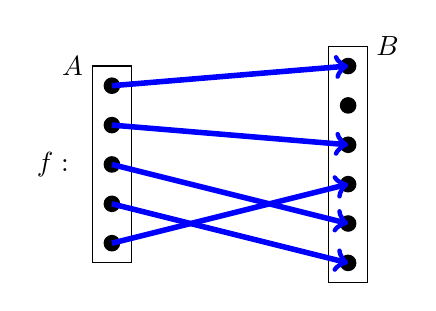
\begin{tikzpicture}
\foreach \x in {1,...,6}
	{\fill[black] (3,0.5*\x-0.5) circle (3pt);}
	%\node at (-0.25,0.5*\x-0.5) {\x};}

\draw (-0.25,0) -- (0.25,0) -- (0.25, 2.5) -- (-0.25,2.5) -- (-0.25,0);

\foreach \x in {1,...,5}
	{\fill[black] (0,0.5*\x-0.25) circle (3pt);}
	%\node at (3.25,0.5*\x-0.25) {\x};}
	
\draw (2.75,-0.25) -- (3.25,-0.25) -- (3.25, 2.75) -- (2.75,2.75) -- (2.75,-0.25);

\draw[line width=2pt,blue,->] (0,0.25) -- (3,1);
\draw[line width=2pt,blue,->] (0,0.75) -- (3,0);
\draw[line width=2pt,blue,->] (0,1.25) -- (3,0.5);
\draw[line width=2pt,blue,->] (0,1.75) -- (3,1.5);
\draw[line width=2pt,blue,->] (0,2.25) -- (3,2.5);

\node at (-0.5,2.5) {$A$};
\node at (3.5,2.75) {$B$};

\node at (-0.75,1.25) {$f:$};
\end{tikzpicture}
\end{figure}
\column{0.5\textwidth}
\begin{figure}
\centering
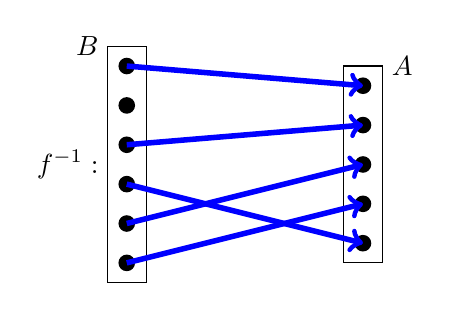
\begin{tikzpicture}
\foreach \x in {1,...,6}
	{\fill[black] (0,0.5*\x-0.5) circle (3pt); }
	%\node at (-0.25,0.5*\x-0.5) {\x};}

\draw (-0.25,-0.25) -- (0.25,-0.25) -- (0.25, 2.75) -- (-0.25,2.75) -- (-0.25,-0.25);

\foreach \x in {1,...,5}
	{\fill[black] (3,0.5*\x-0.25) circle (3pt);}
	%\node at (3.25,0.5*\x-0.25) {\x};}
	
\draw (2.75,0) -- (3.25,0) -- (3.25, 2.5) -- (2.75,2.5) -- (2.75,0);

\draw[line width=2pt,blue,->] (0,0) -- (3,0.75);
\draw[line width=2pt,blue,->] (0,0.5) -- (3,1.25);
\draw[line width=2pt,blue,->] (0,1) -- (3,0.25);
\draw[line width=2pt,blue,->] (0,1.5) -- (3,1.75);
%\draw[line width=2pt,blue,->] (0,2) -- (3,2.25);
\draw[line width=2pt,blue,->] (0,2.5) -- (3,2.25);

\node at (-0.5,2.75) {$B$};
\node at (3.5,2.5) {$A$};

\node at (-0.75,1.25) {$f^{-1}:$};

\end{tikzpicture}
\end{figure}
\end{columns}\vspace{0.2cm}
So this doesn't work. In order to rule this out, we introduce the following notion.
\bl[Definition]{Let $f:A\to B$. We say that $f$ is \textbf{onto} $B$ provided that for every $b\in B$, there is an $a\in A$ so that $f(a)=b$. In other words, $\textrm{im}f=B$.}
\end{frame}

\begin{frame}
Let $A=\{1,2,3,4,5,6\}$ and $B=\{7,8,9,10\}$ and
\[
f=\{(1,7),(2,7),(3,8),(4,9),(5,9),(6,10)\},
\]
\[
g=\{(1,7),(2,7),(3,7),(4,9),(5,9),(6,10)\}.
\]
Then $f: A\to B$ is onto, but $g:A\to B$ is not onto!

\bl[Proving a function is onto]{
To show $f:A\to B$ is onto:
\itemb
\item \textbf{Direct method:} Let $b$ be an arbitrary element of $B$. Explain how to find/construct and element $a\in A$ such that $f(a)=b$. Therefore $f$ is onto.
\item \textbf{Set method:} Show that the sets $B$ and $\textrm{im}f$ are equal.
\iteme}
\end{frame}

\begin{frame}
\bl[Example]{Let $f:\mathbb{Q}\to\mathbb{Q}$ be defined by $f(x)=3x+4$. Prove that $f$ is onto $\mathbb{Q}$.}
\begin{proof}
Let $b\in\mathbb{Q}$ be arbitrary. We seek an $a\in\mathbb{Q}$ such that $f(a)=b$. Let $a=\frac{1}{3}(b-4)$. Since $b$ is a rational number, so is $a$. Notice that
\[
f(a)=3\left[\frac{1}{3}(b-4)\right]+4=(b-4)+4=b.
\]
Therefore $f:\mathbb{Q}\to\mathbb{Q}$ is onto.
\end{proof}
Now we answer the question:
\bl[Theorem]{Let $A$ and $B$ be sets and let $f:A\to B$. The inverse relation $f^{-1}$ is a function from $B$ to $A$ if and only if $f$ is one to one and onto.}
\end{frame}

\begin{frame}

\bl[Definition]{Let $f:A\to B$. We call $f$ a \textbf{bijection} provided it is both one-to-one and onto.}

\bl[Example]{ Let $A$ be the set of even integers and let $B$ be the set of odd integers. The function $f:A\to B$ defined by $f(x)=x+1$ is a bijection.}

\bl[Proof]{
\only<1>{To show that $f$ is one to one, suppose $f(x)=f(y)$ where $x$ and $y$ are even integers. Thus
\[
f(x)=f(y)\qquad\Rightarrow \qquad x+1=y+1\qquad\Rightarrow \qquad x=y.
\]
Hence $f$ is one-to-one.
[...]}
\only<2>{To see that $f$ is onto $B$, let $b\in B$. By definition $b=2k+1$ for some $k\in\mathbb{Z}$. Let $a=2k$; clearly $a$ is even. Then 
\[
f(a)=a+1=2k+1=b
\]
so $f$ is onto. \\
~~~~Since $f$ is both one-to-one and onto, $f$ is a bijection.\qed}
}

\end{frame}

\begin{frame}
\center Do Problems 5-6 on the worksheet.
\end{frame}
\end{document}